

\section{Our Framework}
\label{sec:framework}
In this section, we present our proposed method \ClusterEA{}, a novel scalable EA framework. We start with the overall framework, followed by details on each component of our framework.

\subsection{Overall Framework of \ClusterEAplain{}}

\begin{figure*}[t]
% \vspace{-1mm}
\centering
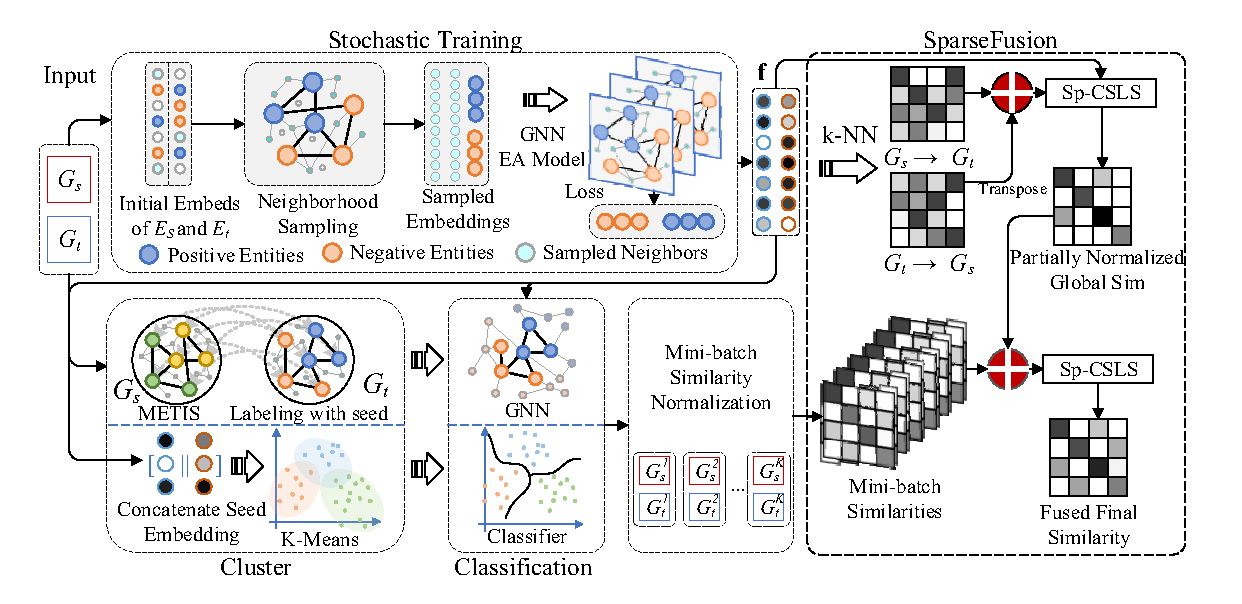
\includegraphics[width=6.in]{figs/framework.eps}
\vspace{-2mm}
\caption{The overall \ClusterEAplain{} framework}
\label{fig:framewrok}
\vspace*{-4mm}
\end{figure*}

As shown in Figure~\ref{fig:framewrok}, to scale up GNN training over large-scale KGs, \ClusterEA{} first utilizes neighborhood sampling~\cite{GraphSAGE17} to train a large-scale GNN for EA in a stochastic fashion.
Thereafter, \ClusterEA{} proposes a novel learning-based batch sampling strategy \Sampling{}. It uses the embedding vectors obtained from stochastic training. In the strategy, two batch samplers that learn multiple aspects of the input KGs are applied to the input KGs, including
(i) \MetisGCN{} that aims at retaining the intra-KG graph structure information such as the neighborhood of nodes, and
(ii) \KMeans{} that aims at retaining the inter-KG matching information provided by the learned embedding.
These methods sample two KGs into multiple mini-batches with a high entity equivalent rate that better satisfies the 1-to-1 mapping assumption.
Finally, \ClusterEA{} proposes \Merging{}, which fuses the normalized local similarity matrices with partially normalized global similarity. The \Merging{} produces the fused final matrix with high sparsity while keeping as much valuable information as possible.

% \vspace{-3mm}
\subsection{Stochastic Training of GNNs for EA}
\label{sec:mini-batch-training}

GNN-based methods \cite{AttrGNN20,KECG19, EVA20, AliNet20, DualAMN21} have dominated the EA tasks with promising performances by propagating the information of seed alignments to their neighbors.
Inspired by this, we propose to incorporate GNN-based models into \ClusterEA{}.
\ClusterEA{} provides a general framework for training a Siamese GNN on both $G_s$ and $G_t$ that all GNN-based EA models follow. As a result, any existing GNN model can be used in \ClusterEA{} to produce the structural feature embeddings of entities.

To scale up the existing GNN-based EA models, \ClusterEA{} trains the models with neighborhood sampling. We sample mini-batches based on the seed alignment. Specifically, following the negative sampling process, we first randomly select a mini-batch of size $N_p$ containing source and target entities $\phi_s'$ and $\phi_t'$ in the seed alignment $\phi^{\prime}$ that are equivalent. Then, randomly sample source and target entities size of $N_n$ with seed alignment in their whole entity sets that does not overlap with selected seed entities, denoted as $\theta_s = \{e_s |e_s \in E_s \cap e_s \not\in \phi_s'\}$ and $\theta_t = \{e_t |e_t \in E_t \cap e_t \not\in \phi_t'\}$. Finally, a mini-batch $B = \{B_s, B_t\} = \{(\phi_s' \cup \theta_s), (  \phi_t' \cup \theta_t) \}$ is generated waiting for the GNN model to produce its embeddings.

Generally, the GNN-based models train the entity's embedding by propagating the neighborhood information~\cite{RREA20, GCN17, GAT18}.
Formally, the embedding of an entity $v \in B$ in the $k_{th}$ layer of GNN $h_v^k$ is obtained by aggregating localized information via

\vspace{-3mm}
\begin{equation}
\begin{array}{c}
a_{v}^{(k)}=\operatorname{Aggregate}^{(k)}(\left\{h_{u}^{(k-1)} \mid u \in \mathcal{N}(v)\right\}) \\
h_{v}^{(k)}=\operatorname{Update}^{(k)}(a_{v}^{(k)}, h_{v}^{(k-1)})
\end{array}
\label{eq:message_passing}
\end{equation}
% \begin{gather}%RREA
% \bm{h}_{\mathcal{N}_{e_{i}}^{e}}^{l} \leftarrow f(\{\bm{h}_{e_{k}}^{l}, \forall e_{k} \in\left\{e_{i}\right\} \cup \mathcal{N}_{e_{i}}^{e}\})\\
% \bm{h}_{e_{i}}^{l+1} \leftarrow \sigma(\bm{W}^{l} \cdot \bm{h}_{\mathcal{N}_{e_{i}}^{e}}^{l})
% \end{gather}
% Here, $f(\cdot)$ is;
where $h_v^0 \in \mathcal{R}^D$ is a learnable embedding vector initialized with Glorot initialization, and 
$\mathcal{N}(v)$ represents the set of neighboring entities around $v$. The model's final output on entity $e$ is denoted as $\mathbf{f}_e$. By applying neighborhood sampling, the size of neighborhood of each entity is limited that no more than a fan out hyperparameter $F$, formally $|\mathcal{N}(v)|\leq F$. We place the graph information on CPU memory. When computing one layer of GNN in each batch, the neighbor of entities in current batch is sampled to form a block of graph, the graph information of this block will be transferred to GPU memory, along with the computation graph, making the final loss backward propagated with GPU.

To maximize the similarities of equivalent entities in each mini-batch, GNN-based EA models often use triplet loss along with negative sampling~\cite{GCN-Align18, KECG19, RREA20, MRAEA20}. In this paper, the \emph{Normalized Hard Sample Mining (NHSM)} loss~\cite{DualAMN21}, an extension for negative sampling that could significantly reduce training epochs, is adopted by us for training large-scale GNNs. We detail how we apply the NHSM loss in Appendix~\ref{app:nhsm}.


\noindent
\textbf{Discussions.}
Due to the neighborhood sampling process, our stochastic version of EA training will have a certain graph information loss, which is minimized with the randomness of sampling. Recent studies~\cite{ClusterGCN} have proposed to limit the sampling in small fixed sub-graphs for better training speed, which will further decrease the accuracy.
LargeEA~\cite{LargeEA22}, on the other hand, trains multiple GNNs on small batches generated with a rule-based method. Such an approach could fasten the training process. Nonetheless, much of the structure information is lost during partitioning, incurring poor performance. Although LargeEA can scale up the EA models to deal with large-scale datasets, it has too much trade-off on the accuracy, which is unreasonable.
% $\mu(e_{i}, e_{j})=\frac{1}{\left|E_{2}\right|} \sum_{e_{j}^{\prime} \in E_{2}} l_{o}(e_{i}, e_{j}, e_{j}^{\prime})$ and $\sigma^{2}(e_{i}, e_{j})=\frac{1}{\left|E_{2}\right|} \sum_{e_{i}^{\prime} \in E_{2}}\left[l_{o}(e_{i}, e_{j}, e_{j}^{\prime})-\mu(e_{i}, e_{j})\right]^{2}$ are the mean and variance of the loss of current batch.


% Formally, $\mathcal{L}=\sum\nolimits_{(e_s^{i}, e_t^{i'}) \in \phi'} \left[f_p(\bm{h}_{e_s^{i}},\bm{h}_{e_{t}^{i'}}) + \gamma - f_n(\bm{h}_{e_s^{i}},\bm{h}_{e_{t}^{i'}}) \right]_{+}$.
% Here,
% $\bm{h}_{e_s^{i}}$ and $\bm{h}_{e_{t}^{i'}}$ represent the embeddings of $e_s^{i}$ and $e_t^{i'}$ learned by a structure-based EA model, respectively;
% $f_p(\cdot,\cdot)$ represents the distance between $\bm{h}_{{e}_{s}^{i}}$ and $\bm{h}_{{e}_{t}^{i'}}$;
% $f_n(\cdot,\cdot)$ denotes the distance of a negative entity pair derived from $e_s^{i}$ and $e_t^{i'}$, generated by replacing either $\bm{h}_{{e}_{s}^{i}}$ or $\bm{h}_{{e}_{t}^{i'}}$ with a new embedding according to the nearest neighbor sampling~\cite{RREA20}; $[x]_{+} = max\{0,x\}$; and
% $\gamma > 0$ is a margin hyper-parameter.


% We denote $\bm{M_s}$ the total structure-based entity similarity matrix, where each value is computed by the Manhattan distance.
% %
% %We would like to highlight that
% $\bm{M_s}$ is highly sparse.
% With independent mini-batch training, all non-zero similarity values lie on the diagonal blocks of $\bm{M_s}$.
% It saves memory cost for coping with large-scale EA. The memory cost of storing $\bm{M_s}$ is $\mathcal{O}(|E_s|)$, i.e., the number of entities in the source KG.
% The time and space complexities of the entire mini-batch training process are $O\left (|\phi'|\times(|T_s|+|T_t|))$ and $O(|D_{str}|\times(|E_s| + |E_t|) + |T_s| + |T_t|)$, respectively.
% Here, $|D_{str}|$ denotes the dimension of every entity embedding learned by the mini-batch training.

\vspace{-3mm}
\subsection{Learning-based Mini-batch Samplers}


% \begin{figure}[t]
% % \vspace*{-18mm}
% \centering
% % \includegraphics[width=6.2in]{METIS-CPS-example.eps}
% 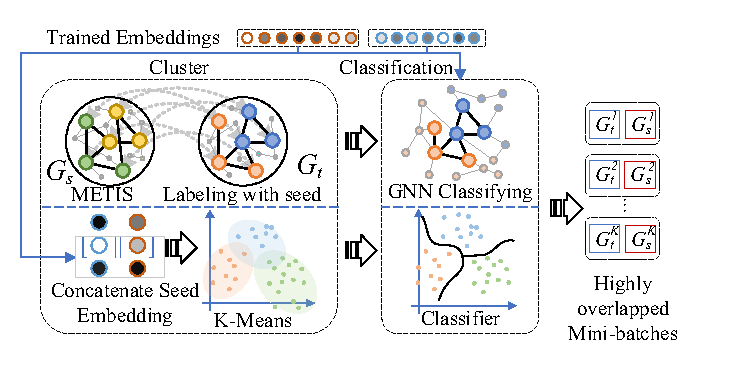
\includegraphics[width=3.5in]{figs/cluster_sampler.eps}
% \vspace*{-2mm}
% \caption{A toy example of \Sampling{} workflow.}
% \label{fig:metis-cps}
% % \vspace*{-2mm}
% \end{figure}
After obtaining the KG embeddings, we aim to build batch samplers that utilize the features learned by EA models for generating mini-batches with high entity equivalent rate. To this end, we present the \Sampling{} strategy, which first \emph{clusters} the training set for obtaining batch labels, and then fits a \emph{classification} model with train labels to put all the entities into the right batch. The two models must satisfy two rules: (i) \emph{scalability} that both the classification and clustering method should be able to apply on large-scale data; and (ii) \emph{distinguishability} that the classifier must be able to distinguish entities into different labels the clustering method provides. If the \emph{scalability} rule is not satisfied, the model will crash due to limited computing resources. If the \emph{distinguishability} rule is not satisfied, the model cannot produce reasonable output. For example, if we randomly split the train set, there is no way for any model to classify the entities with such a label. Following the two rules, by changing different clustering and classification methods, we propose two batch samplers capturing different aspects of information in the two KGs. Each of them produces a set
containing $K$ batches. To distinguish them from batches in Section~\ref{sec:mini-batch-training}, the batches are denoted as $\mathcal{B} = \{(\mathcal{B}_s, \mathcal{B}_t)\}$, where $\mathcal{B}_s \subset E_s$ and $\mathcal{B}_t \subset E_t$ are the sets of source and target entities respectively for each batch. 


\noindent
\textbf{Mini-batch sampling with Intra-KG information.} In the \Sampling{} strategy, we first present  \MetisFullName{} (\MetisGCN{}) for sampling batches based on learning neighborhood information of KGs. Following the  \emph{distinguishability} rule, for retaining the neighborhood information, the clustering method should put nodes that are neighbors into the same batch. This brings us to minimize the edge cut. A previous study proposes METIS-CPS~\cite{LargeEA22}, which clusters two KGs with METIS~\cite{METIS98}, a classic algorithm to partition large graphs for minimizing the edge cut. METIS-CPS is designed to minimize both the edge cuts of two KGs and the decrease of entity equivalent rate. It first clusters source KG with METIS, and then clusters target KG with higher weights set for train nodes guiding the METIS algorithm. However, it has a major flaw: the METIS algorithm on the target KG is also a clustering algorithm. It does not necessarily follow the guidance of train nodes. Following the \Sampling{} strategy, \MetisGCN{} also adopts METIS for \emph{clustering} source KG, but trains a GNN~\cite{GCN17} for \emph{classifying} target KG. The labels provided by METIS will keep nodes that neighbor together as much as possible, and thus can be learned with neighborhood propagation of GNNs. The training and inference on target KG could follow standard node classification task settings. For scalability consideration, we adopt the classic GCN as the classification model. We use the learned embeddings $\mathbf{f}$ of the EA model as the input feature and cross-entropy as the learning loss to train a two-layer GCN. Since GCN does not recognize different relation types in KGs, we adopt the computation of weights in the adjacency matrix from GCN-Align~\cite{GCN-Align18} to convert triples with different relation types into different edge weights. We detail the adjacency matrix construction in Appendix~\ref{app:adj-matrix}.

\noindent
\textbf{Mini-batch sampling with Inter-KG information.} Recall that the cross-KG mapping information is learned into two sets of embeddings $\mathbf{f}_s$ and $\mathbf{f}_t$, partitioning based on these embeddings could preserve the mapping information as much as possible. We propose \KMeansFullName{} (\KMeans{}) for partitioning directly based on the embedding vectors.
For obtaining labels of training sets, in \emph{clustering} process of \KMeans{}, we adopt the K-Means algorithm, a widely-used and scalable approach to cluster embeddings in high-dimensional vector spaces.
K-Means may lead to the entities unevenly distributed in different batches. To reduce this effect and to obtain more balanced mini-batches, we normalize the entity features with the standard score normalization. We concatenate the normalized embeddings of the training set into one unified set of embeddings. Then, we cluster the embeddings to obtain the labeled batch number for the training set $C'$. Formally,

% \vspace{-2mm}
\begin{equation}
\begin{array}{c}
    C'_{e_s} = C'_{e_t} = \operatorname{k-Means}(\mathbf{f}_{n}(e_s,e_t), K), \; (e_s, e_t) \in \phi'\\
    \mathbf{f}_{n}(e_s,e_t)= [\operatorname{z-score}(\mathbf{f}_{e_s})||\operatorname{z-score}(\mathbf{f}_{e_t})]
\end{array}
\end{equation}
where $K$ is the number of mini-batches, and $\operatorname{z-score}(X)=  \frac{X - \mu(X)}{\sigma(X)}$ is the standard score normalization.

Next, we use the label to train two classifiers for both $E_s$ and $E_t$, and predict on all the embeddings. We describe how to obtain the batch number of each entity as follows: $C_{E_s} = \{ \operatorname{clf}(\mathbf{f}_{\phi'_s}, C'_{\phi'_s}, \mathbf{f}_{e_s}) \;|\; e_s \in E_s \}$ and $
    C_{E_t} = \{ \operatorname{clf}(\mathbf{f}_{\phi'_t}, C'_{\phi'_t}, \mathbf{f}_{e_t}) \;|\; e_t \in E_t \}$, 
% \MARK{fix equation here}
% !TODO fix eq
% \vspace{-2mm}
% \begin{equation}
% \begin{array}{c}
%     C_{E_s} = \{ \operatorname{clf}(\mathbf{f}_{\phi'_s}, C'_{\phi'_s}, \mathbf{f}_{e_s}) \;|\; e_s \in E_s \}\\
%     C_{E_t} = \{ \operatorname{clf}(\mathbf{f}_{\phi'_t}, C'_{\phi'_t}, \mathbf{f}_{e_t}) \;|\; e_t \in E_t \}
% \end{array}
% \end{equation}
where $\operatorname{clf}(\mathbf{f}_{train}, C_{train}, \mathbf{f})$ denotes the classification model. It trains based on the training set embedding $\mathbf{f}_{train}$ and label $C_{train}$, and then, it predicts the class for embedding $\mathbf{f}$. In this paper, we use XGBoost Classifier~\cite{XGBoost16}, a scalable classifier that has been a golden standard for various data science tasks. After classification, we can easily obtain the batches with the label $C$.

\subsection{Fusing Local and Global Similarities}

Since the \Sampling{} strategy utilizes different aspects of information to learn the mini-batches, the mini-batch similarity matrices generated may be biased by the corresponding batch sampler. For example, \KMeans{} only relies on the embeddings, tending to put entities with similar embeddings together. This information bias may have a negative effect on the final accuracy. To avoid such bias as much as possible, we propose \Merging{}. It first applies Sinkhorn iteration on mini-batch similarity matrices generated by multiple batch samplers. Then, \Merging{} sums all the similarity matrices of generated batches to obtain a fused local similarity matrix. Finally, it further fuses the local similarity matrix with a partially normalized global similarity based on a newly proposed sparse version of CSLS~\cite{CSLS}, namely, \SparseCSLS{}.


\noindent
\textbf{Local Similarity Matrix Normalization.}
\label{sec:normalize-local-sim}
Previous section describes how to sample the input KGs into multiple batches. For each batch generated from a batch-sampler $\mathcal{B}^i \in \mathcal{B} = \{\mathcal{B}^i_s, \mathcal{B}^i_t\}, i \in K$,  we assume that there exists 1-to-1 mapping between the source and target entities. We first obtain the local similarity matrix $\mathcal{M}^i\in \mathcal{R}^{|E_s|\times|E_t|}$ of current batch.
Formally,

\vspace{-2mm}
\begin{equation}
   \mathcal{M}^i_{e_s, e_t}  =
    \begin{cases}
      \operatorname{sim}(e_s, e_t) & \text{if $e_s \in \mathcal{B}^i_s$ and $e_t \in \mathcal{B}^i_t$}\\
      0 & \text{otherwise}
    \end{cases}
\end{equation}
% \vspace{-2mm}
% $\mathcal{M}^i_{e_s, e_t} = \operatorname{sim}(e_s, e_t)$, $e_s \in \mathcal{B}^i_s$ $e_t \in \mathcal{B}^i_t$.
where $\operatorname{sim}(e_{s}, e_{t})= \mathbf{h}_{e_s} \cdot \mathbf{h}_{e_t}$ is the similarity of two entities obtained with the GNN output feature.

Then, we follow~\cite{Sinkhorn13} to implement the Sinkhorn iteration. We iteratively normalize the similarity matrix $K_s$ rounds in each batch, converting the similarity matrix into a doubly stochastic matrix.
The entities of mini-batches in one graph do not have overlap with each other, meaning that there will be no overlapped values in all the mini-batch similarities. Therefore, to obtain the locally normalized similarity for the whole dataset, we directly sum up all the mini-batch similarities, denoted as $\mathcal{M} = \sum_{i \in K} \operatorname{Sinkhorn} (\mathcal{M}^i, K_s) \in [0,1] ^{|E_s|\times|E_t|}$.
% \begin{equation}
%     \hat{\mathcal{M}}^i = \operatorname{Sinkhorn} (\mathcal{M}^i, K_i)
% \end{equation}

\noindent
\textbf{Fusing multi-aspect local similarities.}
To avoid the bias from one batch sampler, we calculate multiple similarity matrices as described above with different batch samplers. We obtain the cross-KG information-based similarity $\mathcal{M}_C$ with \KMeans{}, and intra-KG information-based similarity $\mathcal{M}_I$ with \MetisGCN{}.
Since the \MetisGCN{} process is unidirectional, indicating that this process on $G_s \rightarrow G_t$ produces different result with $G_t \rightarrow G_s$. According to this characteristic, we apply \MetisGCN{} on both direction, resulting into two matrices $\mathcal{M}_{I, G_s\rightarrow G_t}$ and $\mathcal{M}_{I, G_t\rightarrow G_s}$. Following~\cite{CEAFF20}, we sum up all the similarity matrices without setting any weight to obtain the final local similarity matrix. Formally, $ \mathcal{M}_{L} = \mathcal{M}_C + \mathcal{M}_{I, G_s\rightarrow G_t}+ \mathcal{M}_{I, G_t\rightarrow G_s}^T$.
This simple approach of fusing multi-view similarity matrices is proved to be useful in various previous studies~\cite{CEAFF20, CEAFF21, EASY21, LargeEA22}.

\noindent
\textbf{Normalize global similarity with \SparseCSLS{}.} To fuse the normalized local similarity matrix $\mathcal{M}_{L}$ with the global similarity, we first obtain the global similarity, and normalize it partially.
A widely-used normalization approach for solving geometric problems is to apply CSLS~\cite{CSLS} on the similarity matrix.
Formally, for two entities $e_s$ and $e_t$,
$\operatorname{CSLS}(e_s, e_t) = 2\operatorname{sim}(e_s, e_t) - r_S(e_t) - r_T(e_s)$, where $r_S$ and $r_T$ are the nearest neighborhood similarity mean, which can be obtained by k-NN search with $K_n$ as the neighborhood size.

% \begin{align}
%     \operatorname{CSLS}(x_{s}, y_{t}) =2 \operatorname{sim} (x_{s}, y_{t})-r_{T}( x_{s})-r_{S}(y_{t})
% \end{align}
% where $r_{T}(x_{s}) =\frac{1}{K} \sum_{y \in N_{T}( x_{s})} \operatorname{sim} (x_{s}, y_{t})$ is used to denote the mean neighborhood similarity, the $r_T$.
% on this bi-partite graph, associated with a mapped source word embedding Wxs. All K elements of NT(Wxs) are words from the target language.
% \begin{align}
    %  r_{T}(x_{s}) =\frac{1}{K} \sum_{y \in N_{T}( x_{s})} \operatorname{sim} (x_{s}, y_{t})
% \end{align}

% Similarly we denote by NS(yt) the neighborhood associated with a word t of the target language. Consider the mean similarity of a source embedding xs to its target neighborhood as
However, CSLS also lack scalability, which motivates us to propose a sparse version of CSLS, i.e., \SparseCSLS{}. Recent studies~\cite{LargeEA22, NoMatch21} apply FAISS~\cite{JDH17} to compute K-nearest neighbours of $E_s$ on the embedding space $\mathbf{h}_t$. Similar to the dense version of CSLS, \SparseCSLS{} normalizes a sparse similarity matrix, resulting in a partially normalized similarity matrix. It first uses FAISS to calculate mean neighborhood similarities  $r_{T}( x_{s})$ and $r_{S}(y_{t})$. Then, for a sparse matrix $\mathcal{M}$, the \SparseCSLS{} only subtracts nonzero values of $2 \mathcal{M}$ with $r_{T}( x_{s})$ and $r_{S}(y_{t})$, the result is denoted as $\mathcal{M}'$. To keep the nonzero values to be useful, the final output is normalized with min-max normalization. Formally, $\operatorname{Sp-CSLS}(\mathcal{M}) =\frac{ \mathcal{M}' - \operatorname{min}(\mathcal{M}')}{ \operatorname{max}(\mathcal{M}') - \operatorname{min}(\mathcal{M}')}$.

To obtain the normalized global similarity. We first utilize FAISS to obtain an initial global similarity matrix by fusing k-NN similarity matrices on both $\mathbf{f}_s \rightarrow \mathbf{f}_t$ and $\mathbf{f}_t \rightarrow \mathbf{f}_s$ directions. Next, we normalize it with \SparseCSLS{}. Formally, $\mathcal{M}_{G} = \operatorname{Sp-CSLS}(\operatorname{k-NN}(\mathbf{h}_s, \mathbf{h}_t,K_r) + \operatorname{k-NN}(\mathbf{h}_t, \mathbf{h}_s,K_r)^T, K_n)$, where $\operatorname{k-NN}(\mathbf{X}, \mathbf{Y},K_r)$ returns the similarity matrix of $\mathbf{X} \rightarrow \mathbf{Y}$ remaining only top-$K_r$ values, and $K_n$ is the neighborhood size for CSLS. Note that the sparse similarity of two directions may have some values overlapped, this overlapped values will become twice the value before. However, it will hardly have negative impact on accuracy since entity pairs that both have high ranking on the another KG are more possible to be correctly aligned~\cite{MRAEA20}.

\noindent
\textbf{Fusing normalized similarities.}
To obtain the fused final similarity matrix, we first fuse the global and local similarities, and then apply the \SparseCSLS{} for further normalization on the final matrix. Formally, $\mathcal{M}_{F}=\operatorname{Sp-CSLS}( \mathcal{M}_L +\mathcal{M}_G, K_n)$.







